\begin{frame}[fragile,label=infoFlowVControlFlow]{information flow and control flow}
\begin{lstlisting}[language=Python,style=smaller]
def f(a, b, c):
    if b > 10:
        y = a
    else:
        y = c
    return y
\end{lstlisting}
\begin{itemize}
\item Q: which is better \ldots
    \begin{itemize}
    \item if we're trying to see if user input makes it to SQL query?
    \item if we're trying to determine if private info goes out over network?
    \end{itemize}
\end{itemize}
\begin{tikzpicture}[overlay,remember picture]
\node[anchor=north east] (main) at ([xshift=-.25cm,yshift=-1cm]current page.north east) {
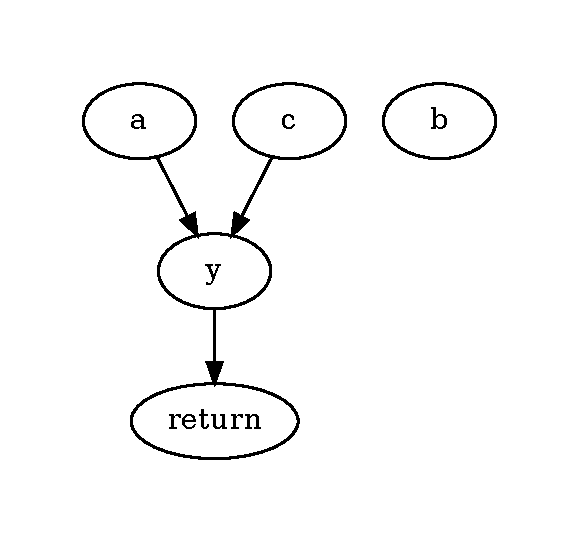
\includegraphics[width=0.3\textwidth]{../taint/info-flow-graph2}
};
\node[anchor=north east] (second) at (main.north west) {
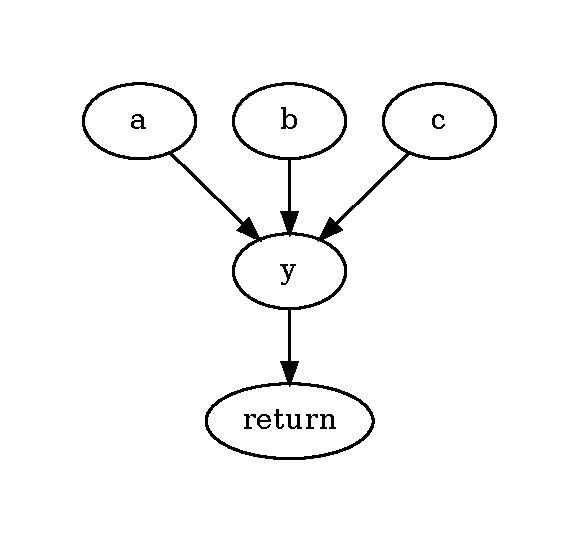
\includegraphics[width=0.3\textwidth]{../taint/info-flow-graph2b}
};
\end{tikzpicture}
\end{frame}
